\leftsection{Исследовательская часть}

\vspace{-1\baselineskip}

\subsection{Технические характеристики}

Технические характеристики устройства, на котором выполнялось тестирование.

\begin{itemize}
    \item Операционная система: Arch~\cite{Arch} Linux 6.12.7~\cite{Linux} x86\_64.
    \item Память: 16 Гб.
    \item Процессор: AMD Ryzen™ 5 4600H CPU @ 3.0G ГГц~\cite{AMD_CPU}.
\end{itemize}

Исследование проводилось на ноутбуке. Во время тестирования
устройство было нагружено только встроенными приложениями окружения.

\subsection{Демонстрация работы приложения}

Для демонстрации работы программы было разработано приложение для удаленного
получения информации о процессах системы. Файл спецификации приведен на
листинге~\ref{lst:example}.

\begin{lstlisting}[caption={Файл спецификации примера}, label={lst:example}]
const NAME_LEN = 16;
const MAX_TASKS = 10;
struct task {
    string name<NAME_LEN>;
    int pid;
    unsigned int state;
    unsigned int flags;
};
typedef struct task tasks<MAX_TASKS>;
program example {
    version initial {
        tasks get_tasks(void) = 1;
    } = 1;
} = 0x20000001;
\end{lstlisting}

\clearpage

Демонстрация работы программы представлена на
рисунках~\refrange{fig:example_call}{fig:example}.

\begin{figure}[!h]
    \centering
    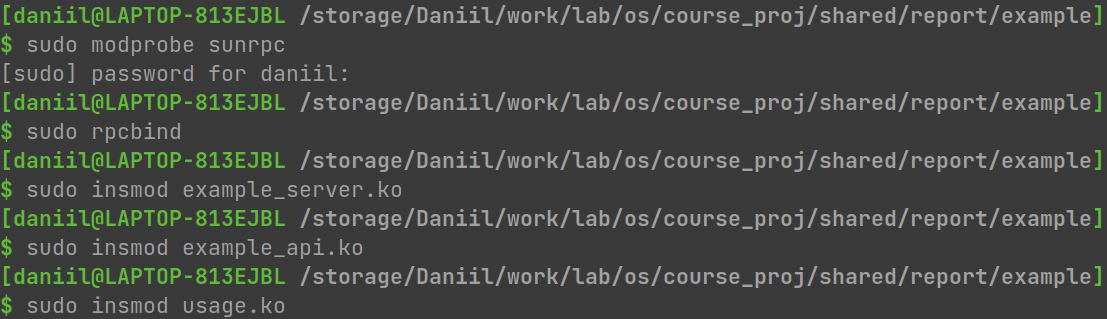
\includegraphics[width=\textwidth]{example_call.png}
    \caption{Последовательность загрузки модулей}
    \label{fig:example_call}
\end{figure}

\begin{figure}[!h]
    \centering
    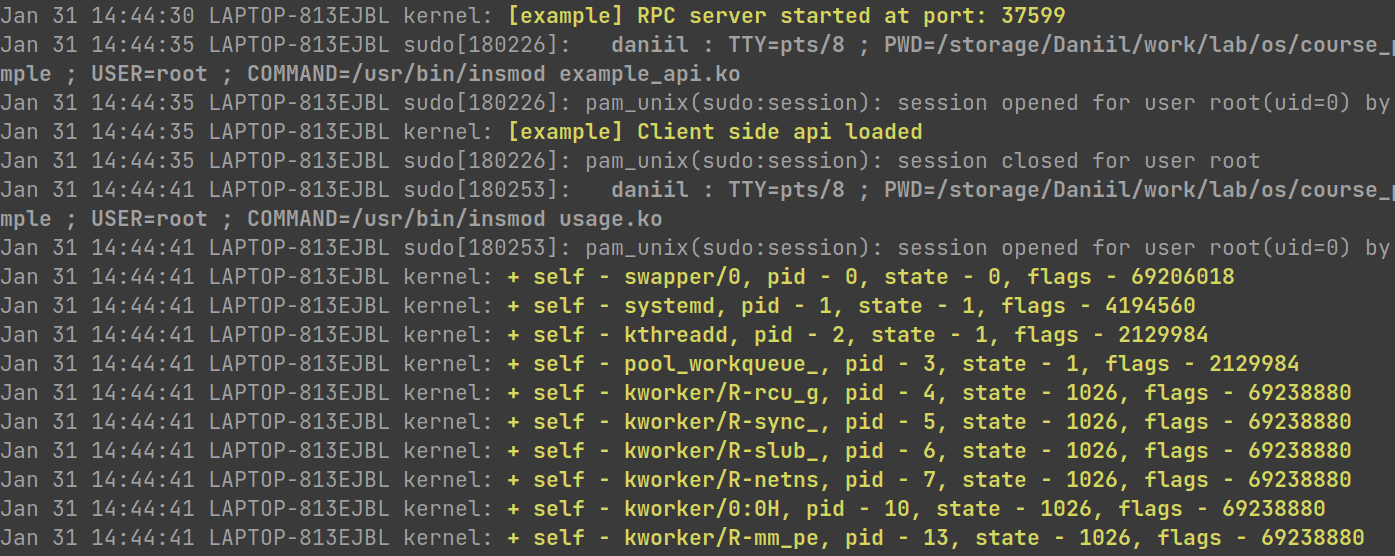
\includegraphics[width=\textwidth]{example.png}
    \caption{Результат работы}
    \label{fig:example}
\end{figure}

\subsection*{Вывод}

В этом разделе был продемонстрирован пример работы приложения-генератора с
последующей загрузкой и исполнением полученного модуля.

